\documentclass{standalone}


\usepackage{amsmath,amssymb,amsfonts}
\usepackage{pgfplots}
\pgfplotsset{width=10cm,compat=1.9}
\pgfplotsset{every axis/.append style={
                     tick label style={font=\footnotesize},
                 }}


\usepgfplotslibrary{fillbetween}
%\usepgfplotslibrary{external}
%\tikzexternalize
\definecolor{darkgreen}{rgb}{0.0, 0.42, 0.24}
\definecolor{amethyst}{rgb}{0.6, 0.4, 0.8}

\begin{document}
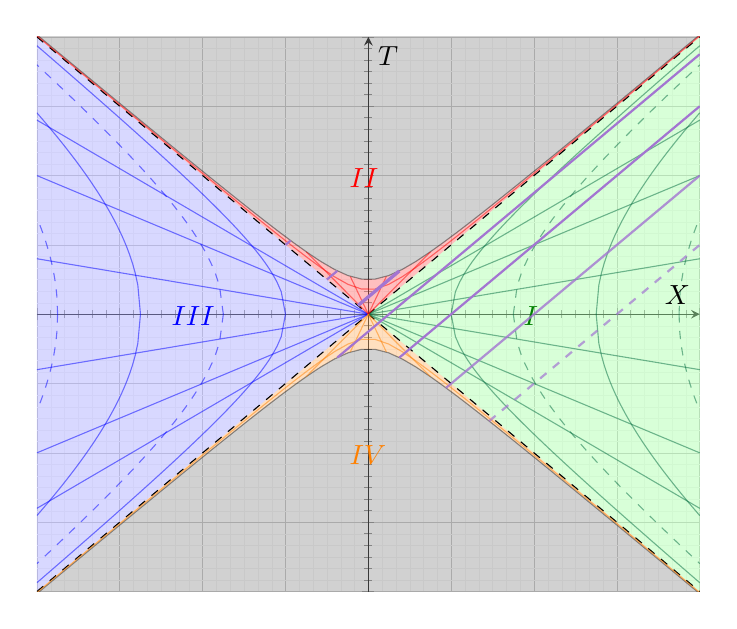
\begin{tikzpicture}
    \begin{axis}[xmin=-8,xmax=8,ymin=-8,ymax=8,
    axis lines=center,
    xlabel=$X$,
    ylabel=$T$,
    yticklabels=false,
    xticklabels=false,
    domain=-8:8,
    minor tick num=5,
    grid=both,
    grid style={line width=.1pt, draw=gray!10},
    major grid style={line width=.2pt,draw=gray!50},
    ]
     \addplot[color=black,dashed, name path=right]{x};  
      \addplot[color=black,dashed, name path=left]{-x};
      % Singulatiry
       \addplot[color=black, samples=50,fill=gray!90,opacity=0.4, name path=upper]{sqrt(x^2+1)}; 
       \addplot[color=black, samples=50,fill=gray!90,opacity=0.4, name path=lower]{-sqrt(x^2+1)};
       % Filling
      \addplot[red!50, opacity=0.5] fill between[of=upper and right, soft clip={domain=0:8}];
      \addplot[red!50, opacity=0.5] fill between[of=upper and left, soft clip={domain=-8:0}];
      \addplot[orange!50, opacity=0.5] fill between[of=lower and left, soft clip={domain=0:8}];
      \addplot[orange!50, opacity=0.5] fill between[of=lower and right, soft clip={domain=-8:0}];
      \addplot[green!30, opacity=0.5] fill between[of=right and left, soft clip={domain=0:8}];
      \addplot[blue!30, opacity=0.5] fill between[of=right and left, soft clip={domain=-8:0}];
      % Labels
      \node[right,thick,color=green!50!black] at (1150,800){$I$};
      \node[right,thick,color=red] at (730,1200){$II$};
      \node[right,thick,color=blue] at (300,800){$III$};
      \node[right,thick,color=orange] at (730,400){$IV$};
      % curved grid lines I
      \addplot[color=darkgreen, opacity=0.5,samples=60,domain=2:8]{sqrt(x^2-2^2)};
      \addplot[color=darkgreen, opacity=0.5,samples=60,domain=2:8]{-sqrt(x^2-2^2)};
      \addplot[color=darkgreen, ,dashed, opacity=0.5,samples=50,domain=3.5:8]{sqrt(x^2-3.5^2)};
      \addplot[color=darkgreen, dashed, opacity=0.5,samples=50,domain=3.5:8]{-sqrt(x^2-3.5^2)};
      \addplot[color=darkgreen, opacity=0.5,samples=40,domain=5.5:8]{sqrt(x^2-5.5^2)};
      \addplot[color=darkgreen, opacity=0.5,samples=40,domain=5.5:8]{-sqrt(x^2-5.5^2)};
      \addplot[color=darkgreen, ,dashed, opacity=0.5,samples=30,domain=7.5:8]{sqrt(x^2-7.5^2)};
      \addplot[color=darkgreen, dashed, opacity=0.5,samples=30,domain=7.5:8]{-sqrt(x^2-7.5^2)};
      \addplot[color=darkgreen, opacity=0.5,samples=10,domain=0:8]{0.7*x};
      \addplot[color=darkgreen, opacity=0.5,samples=10,domain=0:8]{-0.7*x};
      \addplot[color=darkgreen, opacity=0.5,samples=10,domain=0:8]{0.5*x};
      \addplot[color=darkgreen, opacity=0.5,samples=10,domain=0:8]{-0.5*x};
      \addplot[color=darkgreen, opacity=0.5,samples=10,domain=0:8]{0.2*x};
      \addplot[color=darkgreen, opacity=0.5,samples=10,domain=0:8]{-0.2*x};
      %  %  %  %  %  %  %  %  %  % III
      \addplot[color=blue, opacity=0.5,samples=60,domain=-2:-8]{sqrt(x^2-2^2)};
      \addplot[color=blue, opacity=0.5,samples=60,domain=-2:-8]{-sqrt(x^2-2^2)};
      \addplot[color=blue, ,dashed, opacity=0.5,samples=50,domain=-3.5:-8]{sqrt(x^2-3.5^2)};
      \addplot[color=blue, dashed, opacity=0.5,samples=50,domain=-3.5:-8]{-sqrt(x^2-3.5^2)};
      \addplot[color=blue, opacity=0.5,samples=40,domain=-5.5:-8]{sqrt(x^2-5.5^2)};
      \addplot[color=blue, opacity=0.5,samples=40,domain=-5.5:-8]{-sqrt(x^2-5.5^2)};
      \addplot[color=blue, ,dashed, opacity=0.5,samples=30,domain=-7.5:-8]{sqrt(x^2-7.5^2)};
      \addplot[color=blue, dashed, opacity=0.5,samples=30,domain=-7.5:-8]{-sqrt(x^2-7.5^2)};
      \addplot[color=blue, opacity=0.5,samples=10,domain=0:-8]{0.7*x};
      \addplot[color=blue, opacity=0.5,samples=10,domain=0:-8]{-0.7*x};
      \addplot[color=blue, opacity=0.5,samples=10,domain=0:-8]{0.5*x};
      \addplot[color=blue, opacity=0.5,samples=10,domain=0:-8]{-0.5*x};
      \addplot[color=blue, opacity=0.5,samples=10,domain=0:-8]{0.2*x};
      \addplot[color=blue, opacity=0.5,samples=10,domain=0:-8]{-0.2*x};
      %  %  %  %  %  %  %  %  %  % II
      \addplot[color=red, opacity=0.5, samples=50]{sqrt(x^2+0.5)};
      \addplot[color=red, opacity=0.5, samples=10,domain=0:1.5]{1.2*x};
      \addplot[color=red, opacity=0.5, samples=10,domain=0:-1.5]{-1.2*x};
      \addplot[color=red, opacity=0.5, samples=10,domain=0:0.435]{2.5*x};
      \addplot[color=red, opacity=0.5, samples=10,domain=0:-0.435]{-2.5*x};
      %  %  %  %  %  %  %  %  %  % IV
      \addplot[color=orange, opacity=0.5, samples=50]{-sqrt(x^2+0.5)}; 
      \addplot[color=orange, opacity=0.5, samples=10,domain=0:-1.5]{1.2*x};
      \addplot[color=orange, opacity=0.5, samples=10,domain=0:1.5]{-1.2*x};
      \addplot[color=orange, opacity=0.5, samples=10,domain=0:-0.435]{2.5*x};
      \addplot[color=orange, opacity=0.5, samples=10,domain=0:0.435]{-2.5*x};
      %  %  %  %  %  %  %  %  %  % ingoing
      \addplot[color=amethyst!90, very thick ,samples=10, domain=-0.25:0.75]{x+0.5};
      \addplot[color=amethyst!90, thick ,samples=10, domain=-1:-0.75]{x+2};
      \addplot[color=amethyst!90, thick ,samples=10, domain=-2:-1.875]{x+4};
      \addplot[color=amethyst!90, thick ,samples=10, domain=-0.75:8]{x-0.5};
      \addplot[color=amethyst!90, thick ,samples=10, domain=0.75:8]{x-2};
      \addplot[color=amethyst!90, thick ,samples=10, domain=1.875:8,opacity=0.8]{x-4}; 
      \addplot[color=amethyst!90, thick ,samples=10, domain=2.917:8,dashed,opacity=0.7]{x-6}; 
    \end{axis}
\end{tikzpicture} 
\end{document}